%% ====================================================================
\section{Resultados y análisis}
\label{sec:resultados}
%% ====================================================================

Esta sección presenta la evidencia cuantitativa disponible para contrastar el modelo.
Los resultados se separan en seis niveles: gates analíticos H1--H3, comparación bajo
comunicación degradada, baseline MARL-CTDE aprendido, actor neuronal CTDE, validación robótica mediante
escenas CoppeliaSim y extensiones físicas del motor matemático. La lectura combina
resultados positivos y negativos, porque ambos delimitan el régimen de validez de
Smith-QR.

\subsection{Protocolo organizado de validación}

La validación final se organiza como una suite reproducible de protocolos. Cada protocolo
declara una hipótesis o condición extendida, su $H_0$, su $H_1$, la fuente de evidencia,
una métrica observable, un umbral de aceptación y una lectura de estado. Esta
organización evita mezclar afirmaciones de distinta fuerza: los resultados probados por
gates algebraicos, las comparaciones estadísticas y las hipótesis extendidas quedan
separados pero trazados dentro de una misma matriz de evidencia.

La decisión usa tres capas. Primero, si existe prueba matemática o contraejemplo
algebraico, se reporta la refutación de $H_0$ como resultado teórico. Segundo, si hay
repeticiones por semillas, se aplica contraste unilateral o intervalo de confianza
pareado con $\alpha=0{,}05$. Tercero, CoppeliaSim aporta evidencia visual con datos
exportados de escena; esa capa valida plausibilidad robótica, no reemplaza el contraste
estadístico principal.

\begin{figure}[H]
\centering

\includegraphics[width=0.92\textwidth]{figures/fig-validation-suite-summary.png}
\caption{Cobertura de la suite V1. Cada barra resume la fracción de gates superados para
una hipótesis, comparación o extensión del motor matemático.}
\label{fig:validation-suite-summary}
\end{figure}

\begin{table}[H]
\centering
\caption{Matriz inferencial $H_0$/$H_1$ para las hipotesis 1--3. La decision distingue prueba matematica, contraste estadistico y alcance del resultado.}
\label{tab:hypothesis-decision-base-a}
\scriptsize
\begin{tabularx}{\textwidth}{@{}>{\raggedright\arraybackslash}p{0.08\textwidth}>{\raggedright\arraybackslash}p{0.25\textwidth}>{\raggedright\arraybackslash}p{0.25\textwidth}>{\raggedright\arraybackslash}p{0.20\textwidth}>{\raggedright\arraybackslash}X@{}}
\toprule
Prot. & $H_0$ & $H_1$ & Contraste & Decisión y alcance \\
\midrule
H1 & Smith no reproduce water-filling en el caso homogéneo. & Smith converge al reparto water-filling en equilibrio homogéneo. & Equivalencia determinista de pendiente y R2.; n=5 puntos de control; p=n/a; IC95=n/a & $H_0$ refutada por prueba matemática y gate exacto. Válida bajo simetría, comunicación global y payoff homogéneo. \\
H2 & La asignación fluida no genera conflicto entero relevante. & Existen coaliciones fluidas parciales que exigen clearing entero. & Binomial unilateral sobre conflicto fluido-entero.; n=252; p=\textless{}0.001; IC95=n/a & $H_0$ rechazada; el clearing entero queda justificado. Mide necesidad de clearing, no superioridad universal en navegación. \\
H3-A & El precio estático mejora o no empeora a Smith. & Existe régimen estático donde el precio empeora a Smith. & Contraejemplo con IC95 unilateral negativo.; n=20; p=0.013; IC95=[-0.0774, -0.0051] & $H_0$ de mejora universal rechazada. Resultado negativo: no invalida el precio temporal. \\
H3-B & El precio temporal no mejora captura bajo deadlines. & El precio temporal mejora captura bajo déficit y deadlines. & Delta pareado con IC95 positivo.; n=20; p=\textless{}0.001; IC95=[0.0029, 0.0121] & $H_0$ rechazada en el régimen temporal controlado. Válida para urgencia, no para equilibrio estático. \\
\bottomrule
\end{tabularx}
\end{table}

\begin{table}[H]
\centering
\caption{Matriz inferencial $H_0$/$H_1$ para las hipotesis 4--6. La decision separa estadistica experimental y alcance operativo.}
\label{tab:hypothesis-decision-base-b}
\scriptsize
\begin{tabularx}{\textwidth}{@{}>{\raggedright\arraybackslash}p{0.08\textwidth}>{\raggedright\arraybackslash}p{0.25\textwidth}>{\raggedright\arraybackslash}p{0.25\textwidth}>{\raggedright\arraybackslash}p{0.20\textwidth}>{\raggedright\arraybackslash}X@{}}
\toprule
Prot. & $H_0$ & $H_1$ & Contraste & Decisión y alcance \\
\midrule
H4 & Smith original mantiene captura operativa en R3. & Smith original cae por debajo del umbral operativo en R3. & t unilateral contra captura mínima 0.20.; n=20; p=\textless{}0.001; IC95=[0.0650, 0.1427] & $H_0$ rechazada; R3 es régimen de fallo de Smith. Fallo operativo bajo comunicación degradada, no bajo conectividad global. \\
H5 & Smith-QR no mejora captura frente a Smith en R3. & Smith-QR mejora captura frente a Smith en R3. & t pareado unilateral sobre 20 semillas.; n=20; p=\textless{}0.001; IC95=[0.1434, 0.2276] & $H_0$ rechazada; mejora estadísticamente declarable. Declaración limitada a captura de recompensa en R3. \\
H6 & Smith-QR domina también en distancia desperdiciada frente a greedy. & La dominancia de Smith-QR no se extiende a todas las métricas. & t pareado unilateral sobre distancia desperdiciada.; n=20; p=0.600; IC95=[-24.2001, 31.4817] & $H_0$ no rechazada; se reporta límite operativo. Smith-QR es superior en captura, no dominante universal. \\
\bottomrule
\end{tabularx}
\end{table}

\begin{table}[H]
\centering
\caption{Matriz inferencial $H_0$/$H_1$ para las hipotesis 7--9. La decision separa evidencia robotica y MARL.}
\label{tab:hypothesis-decision-base-c}
\scriptsize
\begin{tabularx}{\textwidth}{@{}>{\raggedright\arraybackslash}p{0.08\textwidth}>{\raggedright\arraybackslash}p{0.25\textwidth}>{\raggedright\arraybackslash}p{0.25\textwidth}>{\raggedright\arraybackslash}p{0.20\textwidth}>{\raggedright\arraybackslash}X@{}}
\toprule
Prot. & $H_0$ & $H_1$ & Contraste & Decisión y alcance \\
\midrule
H7 & Las escenas robóticas incumplen despejes mínimos o no exportan datos. & Las escenas robóticas son plausibles y exportan métricas auditables. & Acceptance sampling muestral; sin inferencia poblacional.; n=6; p=n/a; IC95=n/a & $H_0$ muestral refutada; evidencia robótica observacional aceptada. No sustituye hardware ni benchmark estadístico principal. \\
H8 & MARL-CTDE no mejora a una politica proxy ni aporta comparador aprendido. & MARL-CTDE aprende una politica compartida y mejora al proxy en al menos un regimen, sin dominar a Smith-QR. & t pareado unilateral por regimen y contraste global frente a Smith-QR.; n=8 escasez; 24 global; p=\textless{}0.001 / 1.000; IC95=[0.1638, 0.2015]; [-0.2448, -0.0834] & $H_0$ rechazada solo contra el proxy en escasez; no se declara superioridad global. Baseline aprendido real para contraste, no contribucion teorica principal. \\
H9 & El actor neuronal CTDE no aporta evidencia adicional frente al proxy o al CTDE lineal. & El actor neuronal CTDE aprende una politica compartida, mejora al proxy en escasez y reduce coste frente al CTDE lineal sin dominar a Smith-QR. & Contraste pareado por regimen y contraste global frente a Smith-QR.; n=8 escasez proxy; 8 escasez coste; 24 global; p=\textless{}0.001 / 0.035 / 1.000; IC95=[0.1484, 0.1978]; [-14.3657, -0.6450]; [-0.2347, -0.1280] & $H_0$ rechazada solo como baseline neuronal adicional; no se declara superioridad global. Aporta comparacion aprendida real; la contribucion principal sigue siendo Smith-QR y el motor matematico. \\
\bottomrule
\end{tabularx}
\end{table}

\begin{table}[H]
\centering
\caption{Matriz inferencial $H_0$/$H_1$ para las hipotesis 10--12. La decision separa densidad predictiva, motor integrado y cobertura Coppelia.}
\label{tab:hypothesis-decision-base-d}
\scriptsize
\begin{tabularx}{\textwidth}{@{}>{\raggedright\arraybackslash}p{0.08\textwidth}>{\raggedright\arraybackslash}p{0.25\textwidth}>{\raggedright\arraybackslash}p{0.25\textwidth}>{\raggedright\arraybackslash}p{0.20\textwidth}>{\raggedright\arraybackslash}X@{}}
\toprule
Prot. & $H_0$ & $H_1$ & Contraste & Decisión y alcance \\
\midrule
H10 & El peaje de densidad predictiva no reduce congestion frente a Smith-QR. & El peaje de densidad predictiva reduce congestion sin degradar productividad. & Contraste pareado sobre 30 semillas sinteticas.; n=30; p=IC95; IC95=ver gates H10-DENS & $H_0$ rechazada en la campana sintetica de almacen. Valida congestion predictiva en un cuello de botella controlado; no sustituye hardware. \\
H11 & La capacidad wrench no mejora el transporte frente a cardinalidad. & La capacidad wrench reduce residual y mantiene limites de torque, energia y bateria. & Contraste pareado y cotas IC95 sobre 30 semillas.; n=30; p=IC95; IC95=ver gates H11-INT & $H_0$ rechazada para el tramo critico simulado. Campana dinamica sintetica; debe ampliarse con ejecucion Coppelia o hardware. \\
H12 & La validacion Coppelia no cubre los escenarios necesarios. & La validacion Coppelia exporta escenas, camaras y artefactos visuales por escenario. & Acceptance sampling de artefactos generados.; n=10; p=n/a; IC95=n/a & $H_0$ refutada como cobertura de artefactos. Estado fallback\_synthetic\_render; no declara ejecucion headless real. \\
\bottomrule
\end{tabularx}
\end{table}

\begin{table}[H]
\centering
\caption{Matriz inferencial $H_0$/$H_1$ para hipotesis extendidas del motor matematico.}
\label{tab:hypothesis-decision-extended}
\scriptsize
\begin{tabularx}{\textwidth}{@{}>{\raggedright\arraybackslash}p{0.08\textwidth}>{\raggedright\arraybackslash}p{0.25\textwidth}>{\raggedright\arraybackslash}p{0.25\textwidth}>{\raggedright\arraybackslash}p{0.20\textwidth}>{\raggedright\arraybackslash}X@{}}
\toprule
Prot. & $H_0$ & $H_1$ & Contraste & Decisión y alcance \\
\midrule
G3 & Cardinalidad suficiente implica capacidad wrench. & La capacidad efectiva requiere rango y residual wrench. & No aplica; gate algebraico.; n=2 configuraciones; p=n/a; IC95=n/a & $H_0$ refutada por contraejemplo constructivo. Necesario para cargas que requieren torque planar. \\
G4 & Mercado, campo y Hamiltoniano no comparten el mismo déficit. & Las tres capas consumen un déficit común verificable. & No aplica; identidad algebraica.; n=gate algebraico; p=n/a; IC95=n/a & $H_0$ refutada hasta precisión numérica. Depende de las hipótesis del contrato de integración. \\
G5 & La extensión dinámica viola los límites de energía/torque. & La extensión dinámica mantiene energía y torque acotados. & No aplica; gate de estabilidad acotada.; n=gate algebraico; p=n/a; IC95=n/a & $H_0$ refutada en el caso controlado. Falta validar con campañas dinámicas de contacto realista. \\
G6 & El peaje predictivo no cambia rutas congestionadas. & El peaje predictivo anticipa congestión y desvía flujo. & No aplica; gate determinista de ruta.; n=1 escenario controlado; p=n/a; IC95=n/a & $H_0$ refutada en el caso controlado. Hipótesis extendida; requiere campaña de congestión para generalizar. \\
G7 & La batería no altera la asignación económica. & La batería actúa como restricción económica de retornabilidad. & No aplica; gate determinista de payoff.; n=1 escenario controlado; p=n/a; IC95=n/a & $H_0$ refutada en el caso controlado. Debe ampliarse con descarga temporal y rutas a cargador. \\
\bottomrule
\end{tabularx}
\end{table}

\begin{table}[H]
\centering
\caption{Matriz de validacion por hipotesis base. Cada protocolo reporta una magnitud observable, un umbral de aceptacion y el estado del gate.}
\label{tab:validation-suite-v1}
\scriptsize
\begin{tabularx}{\textwidth}{@{}>{\raggedright\arraybackslash}p{0.13\textwidth}>{\raggedright\arraybackslash}p{0.34\textwidth}>{\raggedleft\arraybackslash}p{0.14\textwidth}>{\raggedleft\arraybackslash}p{0.14\textwidth}>{\raggedright\arraybackslash}X@{}}
\toprule
Protocolo & Criterio validado & Observado & Umbral & Estado \\
\midrule
$H_1$-G1 & Smith reproduce water-filling homogeneo: R2 del ajuste & 1.0000 & \textgreater{}= 0.9900 & Pasa \\
$H_1$-G1 & Smith reproduce water-filling homogeneo: pendiente staffing observado/teorico & 1.0000 & \textgreater{}= 0.9900 & Pasa \\
H2-G2 & El clearing entero reduce coaliciones parciales inutiles: reduccion relativa de distancia desperdiciada & 1.0000 & \textgreater{}= 0.2500 & Pasa \\
H3A-G3A & El precio estatico no es una mejora universal: delta de utilidad estatica con precio & -0.0410 & \textless{}= 0.0000 & Pasa \\
H3B-G3B & El precio temporal ayuda con deadlines y deficit persistente: delta de captura antes de deadline & 0.2120 & \textgreater{}= 0.0500 & Pasa \\
H4-R3 & Smith original falla bajo comunicacion R3: entregas medias de Smith & 3.2500 & \textless{}= 4.0000 & Pasa \\
H5-R3 & Smith-QR rescata parcialmente R3: captura media Smith-QR & 0.2893 & \textgreater{} 0.1038 & Pasa \\
H7-ROB & Las escenas roboticas validan plausibilidad geometrica: numero de escenas generadas & 6.0000 & \textgreater{}= 6.0000 & Pasa \\
H7-ROB & Las escenas roboticas validan plausibilidad geometrica: separacion inicial minima humano-robot & 6.2394 & \textgreater{}= 2.0000 & Pasa \\
H7-ROB & Las escenas roboticas validan plausibilidad geometrica: separacion inicial minima robot-rack & 3.3015 & \textgreater{}= 1.0000 & Pasa \\
H8-MARL & MARL-CTDE supera al proxy en escasez: delta de captura frente a proxy & 0.1827 & \textgreater{} 0.0000 & Pasa \\
H8-MARL & MARL-CTDE no domina a Smith-QR globalmente: delta global de captura frente a Smith-QR & -0.1641 & \textless{}= 0.0000 & Pasa \\
H8-MARL & MARL-CTDE aprende una politica compartida: ganancia de objetivo episodico & 0.1480 & \textgreater{}= 0.0500 & Pasa \\
H9-MARL & El actor neuronal supera al proxy en escasez: delta de captura frente a proxy & 0.1731 & \textgreater{} 0.0000 & Pasa \\
H9-MARL & El actor neuronal reduce coste operativo frente al CTDE lineal: delta de distancia desperdiciada en escasez & -7.5053 & \textless{} 0.0000 & Pasa \\
H9-MARL & El actor neuronal no domina a Smith-QR globalmente: delta global de captura frente a Smith-QR & -0.1813 & \textless{}= 0.0000 & Pasa \\
H9-MARL & El actor neuronal CTDE aprende desde retornos episodicos: ganancia de objetivo episodico & 0.0520 & \textgreater{}= 0.0300 & Pasa \\
\bottomrule
\end{tabularx}
\end{table}

\begin{table}[H]
\centering
\caption{Matriz de validacion extendida para capacidad vectorial, dinamica, congestion, bateria y cobertura Coppelia.}
\label{tab:validation-suite-extended}
\scriptsize
\begin{tabularx}{\textwidth}{@{}>{\raggedright\arraybackslash}p{0.13\textwidth}>{\raggedright\arraybackslash}p{0.34\textwidth}>{\raggedleft\arraybackslash}p{0.14\textwidth}>{\raggedleft\arraybackslash}p{0.14\textwidth}>{\raggedright\arraybackslash}X@{}}
\toprule
Protocolo & Criterio validado & Observado & Umbral & Estado \\
\midrule
G3-W & Cardinalidad no implica capacidad wrench: residual de coalicion apiñada & 1.1990 & \textgreater{}= 0.2500 & Pasa \\
G3-W & Distribucion de contacto restaura factibilidad: residual de coalicion distribuida & 2.54e-16 & \textless{}= 1.00e-08 & Pasa \\
G4-INT & Mercado, campo y Hamiltoniano consumen el mismo deficit: error maximo de balance de potencia & 2.22e-16 & \textless{}= 1.00e-09 & Pasa \\
G4-INT & La firma del contorno conecta geometria con torque: torque maximo en cuadrado supereliptico & 0.5240 & \textgreater{}= 0.2500 & Pasa \\
G4-INT & La firma del contorno conecta geometria con torque: torque maximo en rectangulo supereliptico & 1.0856 & \textgreater{}= 0.6500 & Pasa \\
G4-INT & La firma del contorno conecta geometria con torque: torque radial maximo en circulo & 0.0000 & \textless{}= 1.00e-08 & Pasa \\
G5-DYN & El contacto util mantiene esfuerzo dinamico acotado: salto Hamiltoniano normalizado & 0.0430 & \textless{}= 0.1000 & Pasa \\
G5-DYN & El contacto util mantiene esfuerzo dinamico acotado: saturacion maxima de torque & 0.5000 & \textless{}= 0.8500 & Pasa \\
G6-CONG & El peaje predictivo evita congestiones antes del atasco: cambio de ruta por peaje & 1.0000 & = 1.0000 & Pasa \\
G6-CONG & El peaje predictivo evita congestiones antes del atasco: densidad maxima sin peaje & 1.6200 & \textgreater{} 1.0000 & Pasa \\
G7-BAT & La bateria entra como restriccion economica: brecha de payoff por retornabilidad & 0.7500 & \textgreater{}= 0.5000 & Pasa \\
\bottomrule
\end{tabularx}
\end{table}

\begin{table}[H]
\centering
\caption{Matriz de validacion aplicada H10--H12. Cada protocolo reporta evidencia estadistica, dinamica o visual exportable.}
\label{tab:validation-suite-campaigns}
\scriptsize
\begin{tabularx}{\textwidth}{@{}>{\raggedright\arraybackslash}p{0.13\textwidth}>{\raggedright\arraybackslash}p{0.34\textwidth}>{\raggedleft\arraybackslash}p{0.14\textwidth}>{\raggedleft\arraybackslash}p{0.14\textwidth}>{\raggedright\arraybackslash}X@{}}
\toprule
Protocolo & Criterio validado & Observado & Umbral & Estado \\
\midrule
H10-DENS & La densidad predictiva no degrada productividad: captura media con peaje predictivo & 1.0000 & \textgreater{}= 0.9700 & Pasa \\
H10-DENS & La densidad predictiva reduce congestion aplicada: delta pareado de densidad maxima futura & -17.3637 & \textless{} 0.0000 & Pasa \\
H10-DENS & La densidad predictiva reduce congestion aplicada: delta pareado de pasos congestionados frente a Smith-QR & -1.62e+02 & \textless{} 0.0000 & Pasa \\
H11-INT & El motor integrado conserva margen de bateria: cota inferior IC95 de bateria minima & 0.8201 & \textgreater{}= 0.7500 & Pasa \\
H11-INT & El motor integrado mantiene energia acotada: cota superior IC95 de salto Hamiltoniano & 0.2141 & \textless{}= 0.3500 & Pasa \\
H11-INT & El motor integrado mantiene torque acotado: cota superior IC95 de saturacion de torque & 0.4055 & \textless{}= 0.8500 & Pasa \\
H11-INT & El motor integrado reduce residual wrench: delta pareado de residual wrench medio & -0.6351 & \textless{} 0.0000 & Pasa \\
H11-INT & El motor integrado completa el tramo critico: delta pareado de throughput frente a cardinalidad & 0.9667 & \textgreater{} 0.0000 & Pasa \\
H12-COP & La campana Coppelia exporta artefactos visuales: fraccion de escenas con PNG y MP4 & 1.0000 & = 1.0000 & Pasa \\
H12-COP & Las escenas Coppelia tienen camaras de auditoria: fraccion de escenas con camara superior y oblicua & 1.0000 & = 1.0000 & Pasa \\
H12-COP & La campana Coppelia cubre escenarios de validacion: numero de escenas generadas & 10.0000 & \textgreater{}= 10.0000 & Pasa \\
\bottomrule
\end{tabularx}
\end{table}

\begin{table}[H]
\centering
\caption{Comparación principal bajo comunicación R3. Las métricas distinguen productividad de coste operativo.}
\label{tab:validation-suite-r3}
\small
\begin{tabularx}{\textwidth}{@{}>{\raggedright\arraybackslash}Xrrrr@{}}
\toprule
Método & Captura media & IC95 captura & Entregas medias & Distancia desperdiciada \\
\midrule
Centralizado limitado & 0.061 & [0.025, 0.097] & 1.85 & 2.86 \\
Smith & 0.104 & [0.065, 0.143] & 3.25 & 16.86 \\
MARL-proxy & 0.237 & [0.201, 0.273] & 6.75 & 41.59 \\
Greedy local & 0.243 & [0.205, 0.281] & 7.05 & 37.44 \\
Smith-QR & 0.289 & [0.268, 0.311] & 8.25 & 41.08 \\
\bottomrule
\end{tabularx}
\end{table}

\begin{table}[H]
\centering
\caption{Evaluacion congelada del baseline MARL-CTDE aprendido. La lectura separa mejora frente al proxy y dominancia frente a Smith-QR.}
\label{tab:validation-suite-marl-ctde}
\small
\begin{tabularx}{\textwidth}{@{}>{\raggedright\arraybackslash}p{0.20\textwidth}>{\raggedright\arraybackslash}p{0.18\textwidth}rrr>{\raggedright\arraybackslash}X@{}}
\toprule
Escenario & Caso & MARL-CTDE & Proxy & Smith-QR & Lectura \\
\midrule
Comunicacion degradada & R3 sin perdida & 0.238 & 0.238 & 0.313 & empata al proxy en captura \\
Fallo de robot & fallo de cuatro robots & 0.412 & 0.594 & 0.599 & resultado negativo \\
Escasez prioritaria & adversarial & 0.538 & 0.356 & 0.769 & mejora al proxy; no domina a Smith-QR \\
\bottomrule
\end{tabularx}
\end{table}

\begin{table}[H]
\centering
\caption{Evaluacion congelada del actor neuronal MARL-CTDE. La lectura separa actor neuronal, actor lineal, proxy y Smith-QR.}
\label{tab:validation-suite-marl-neural}
\small
\begin{tabularx}{\textwidth}{@{}>{\raggedright\arraybackslash}p{0.18\textwidth}>{\raggedright\arraybackslash}p{0.16\textwidth}rrrr>{\raggedright\arraybackslash}X@{}}
\toprule
Escenario & Caso & Neural & Lineal & Proxy & Smith-QR & Lectura \\
\midrule
Comunicacion degradada & R3 sin perdida & 0.163 & 0.163 & 0.185 & 0.231 & empata al actor lineal \\
Fallo de robot & fallo de cuatro robots & 0.299 & 0.313 & 0.527 & 0.543 & resultado negativo \\
Escasez prioritaria & adversarial & 0.538 & 0.519 & 0.365 & 0.769 & mejora al proxy; no domina a Smith-QR \\
\bottomrule
\end{tabularx}
\end{table}

\begin{table}[H]
\centering
\caption{Contrastes pareados de Smith-QR frente a referencias en R3. La dominancia se declara solo cuando el IC95 del delta queda por encima de cero.}
\label{tab:validation-suite-deltas}
\small
\begin{tabularx}{\textwidth}{@{}>{\raggedright\arraybackslash}Xrrr>{\raggedright\arraybackslash}X@{}}
\toprule
Comparación & Delta medio & IC95 bajo & IC95 alto & Lectura \\
\midrule
Smith-QR vs. Smith & 0.1855 & 0.1434 & 0.2276 & mejora declarable \\
Smith-QR vs. Greedy local & 0.0466 & 0.0047 & 0.0886 & mejora declarable \\
Smith-QR vs. Centralizado limitado & 0.2282 & 0.1891 & 0.2673 & mejora declarable \\
Smith-QR vs. MARL-proxy & 0.0527 & 0.0132 & 0.0923 & mejora declarable \\
\bottomrule
\end{tabularx}
\end{table}


Las Tablas~\ref{tab:hypothesis-decision-base-a}--\ref{tab:hypothesis-decision-extended}
son la lectura inferencial: explicitan qué $H_0$ se refuta, qué $H_0$ no se refuta y
cuándo la evidencia es sólo robótica-observacional. Las
Tablas~\ref{tab:validation-suite-v1}--\ref{tab:validation-suite-extended} muestran los
gates operativos que respaldan esa lectura. H1 y H2 cubren el núcleo de water-filling y
clearing entero; H3 separa el resultado negativo del precio estático de su utilidad
temporal; H4--H6 delimitan la comparación R3; H7 mantiene la validación robótica como
plausibilidad geométrica; H8 introduce MARL-CTDE como baseline aprendido con evaluación
congelada; H9 añade un actor neuronal CTDE compartido; y G3--G7 auditan las extensiones de wrench, motor integrado, torque dinámico,
congestión y batería. Las Tablas~\ref{tab:validation-suite-r3},
\ref{tab:validation-suite-marl-ctde}, \ref{tab:validation-suite-marl-neural}
y~\ref{tab:validation-suite-deltas} fijan el
criterio de comparación: Smith-QR o MARL sólo se declaran superiores cuando el intervalo
de confianza del delta pareado queda completamente por encima de cero.

\subsection{Controles mínimos H1--H3}

El protocolo mínimo reproduce el motor esperado:
H1 obtiene pendiente $1.0000$ y $R^2=1$ en el caso de \emph{water-filling}; H2 reduce el
desperdicio aproximadamente un $32\%$ al activar el \emph{clearing} entero. H3 se separó
en dos partes. H3-A confirma el resultado negativo estático: el precio perturba un
equilibrio que Smith ya resuelve por \emph{water-filling}. H3-B es el ensayo temporal con
llegadas y \emph{deadlines}, que es el único régimen donde el precio puede tener valor
operativo.

\subsection{Smith-QR bajo comunicación degradada}

Se comparó Smith-QR completo contra Smith original bajo la misma comunicación local. La
variante completa incorpora memoria de descriptores, compromiso en ruta, guardia de
\emph{clearing}, patrullaje exploratorio y una proyección de quorum local cuando
$R_{\mathrm{com}}\leq 3.25$. Este último cambio es importante: en R3 se rompe el supuesto
práctico de información distribuida suficiente, así que Smith-QR no intenta forzar el
equilibrio fluido sino cerrar tareas localmente.

\begin{table}[H]
\centering
\caption{Validación R3 con 20 semillas.}
\label{tab:smith-qr-r3}
\small
\begin{tabularx}{\textwidth}{@{}>{\raggedright\arraybackslash}Xrlll@{}}
\toprule
Método & $n$ & Captura de recompensa (IC95) & Entregas & Distancia desperdiciada \\
\midrule
Centralizado con comunicación limitada & 20 & 0.061 [0.025, 0.097] & 1.85 & 2.86 \\
Smith & 20 & 0.104 [0.065, 0.143] & 3.25 & 16.86 \\
Greedy local & 20 & 0.243 [0.205, 0.281] & 7.05 & 37.44 \\
MARL-proxy & 20 & 0.237 [0.201, 0.273] & 6.75 & 41.59 \\
Smith-QR & 20 & 0.289 [0.268, 0.311] & 8.25 & 41.08 \\
\bottomrule
\end{tabularx}
\end{table}

El delta pareado de Smith-QR frente a Smith en R3 es positivo:
$+0.1855$ en captura de recompensa, con IC95 $[0.1434,0.2276]$, y $+5.0$
entregas, con IC95 $[3.80,6.20]$. Frente a greedy local, Smith-QR mantiene un delta de
captura $+0.0466$ con IC95 $[0.0047,0.0886]$; frente al proxy MARL inicial, el delta es
$+0.0527$ con IC95 $[0.0132,0.0923]$. La mejora no debe extrapolarse a todas las
métricas: la distancia desperdiciada media no presenta una ventaja concluyente frente a
greedy o al proxy MARL inicial. La afirmación defendible es más precisa: bajo R3, Smith-QR rescata a
Smith y mejora captura/entregas en esta campaña, pagando un coste operativo que debe
vigilarse con métricas de distancia, energía y batería.

\subsection{MARL-CTDE aprendido}

El baseline MARL se elevó de proxy determinista a política aprendida con entrenamiento
centralizado y ejecución descentralizada. Cada robot usa una función compartida
$Q_\theta(o_i,k)$ para puntuar cargas visibles a partir de observaciones locales:
recompensa normalizada, precio, déficit de quorum, edad de la carga, cercanía, soporte
local, estado de transporte, persistencia de asignación y presión de quorum. Los pesos
$\theta$ se optimizan con retornos episódicos comunes de la flota y después se congelan
para evaluación en semillas separadas.

El resultado H8 es deliberadamente conservador. El entrenamiento aumenta el objetivo
episódico en $+0.1480$, lo que confirma que no se trata de una regla fija disfrazada de
MARL. En evaluación congelada, MARL-CTDE mejora al proxy en escasez prioritaria:
$\Delta=+0.1827$ en captura, con IC95 $[0.1638,0.2015]$. Sin embargo, no domina a
Smith-QR globalmente: el delta agregado frente a Smith-QR es $-0.1641$, con IC95
$[-0.2448,-0.0834]$. La lectura correcta es que MARL-CTDE aporta un competidor aprendido
real y útil para contraste, pero no sustituye el mecanismo analítico Smith-QR en esta
campaña.

\subsection{Actor neuronal CTDE}

El siguiente paso fue sustituir la función lineal $Q_\theta(o_i,k)$ por un actor neuronal
compartido con término lineal residual y una capa oculta. La decisión metodológica es
importante: no se etiqueta como MAPPO/PPO porque el simulador no registra todavía
log-probabilidades por acción para estimar una política de gradiente con clipping. En su
lugar, el actor se entrena con búsqueda centralizada sobre retornos episódicos completos
de la flota y se ejecuta de forma descentralizada con las mismas observaciones locales
que el MARL-CTDE lineal.

El gate H9 muestra una mejora de objetivo de entrenamiento de $+0.0520$ respecto a la
inicialización lineal. En evaluación congelada, el actor neuronal mejora al proxy en
escasez prioritaria con $\Delta=+0.1731$ en captura e IC95 $[0.1484,0.1978]$. Frente al
actor lineal, la mejora de captura en escasez es pequeña y no concluyente
($+0.0192$, IC95 $[-0.0054,0.0439]$), pero sí reduce distancia desperdiciada en ese
régimen: $\Delta=-7.5053$ con IC95 $[-14.3657,-0.6450]$. Globalmente sigue por debajo de
Smith-QR en captura: $\Delta=-0.1813$ con IC95 $[-0.2347,-0.1280]$. Por tanto, el actor
neuronal queda como baseline aprendido más fuerte que el proxy y útil para estudiar
coste operativo, pero no como sustituto de la contribución analítica principal.

\subsection{Resultado negativo: logit no rescata R3}

El resultado con mutación/logit es negativo: añadir exploración estocástica a Smith no
basta para resolver la parálisis de comunicación
degradada. La mejor variante explorada no supera de forma limpia a las referencias
locales fuertes, y el hallazgo refuerza la decisión de diseñar Smith-QR como mecanismo
de quorum y comunicación, no como simple ruido exploratorio sobre la dinámica
poblacional.

\subsection{CoppeliaSim industrial}

Se generaron seis escenas reproducibles: nominal con
Smith-QR, R3 con Smith, R3 con Smith-QR, fallo de robot, cruce de humanos y sensores
degradados. Cada escena parametriza suelo industrial, racks, estaciones, cargas,
operadores humanos, zonas ciegas, comunicación local y robots Pioneer~3-DX o una base
diferencial equivalente. Las métricas offline quedan
definidas para distancia mínima, colisión, saturación y eventos de quorum. La separación
inicial mínima humano--robot es $6.24$ m y robot--rack $3.30$ m.

Estas escenas funcionan como entorno de integración robótica: conectan el modelo
matemático con geometría industrial, sensores, comunicación local y riesgos de
seguridad.

\subsection{Métricas dinámicas de capacidad efectiva}

La validación dinámica incorpora métricas físicas que no aparecen en una asignación por
cardinalidad. Las figuras
\ref{fig:port-hamiltoniano-ruedas}, \ref{fig:energia-saltos} y
\ref{fig:carga-rectangular-roles} convierten la hipótesis física en variables
medibles: energía port-Hamiltoniana $H(t)$, energía disipada $E_D$, esfuerzo de rueda
$E_{\tau}$, par máximo $\tau_{\max}$, salto energético $\Delta H$ y separación mínima
real $d_{\min}^{\mathrm{real}}$. Estas métricas permiten detectar un caso especialmente
peligroso para la tesis: una coalición que parece correcta por throughput y factibilidad,
pero que requiere pares no realistas o produce saltos de energía grandes al cambiar de
rol.

La comparación clave de la extensión es cardinalidad mínima frente a capacidad efectiva.
El resultado defendible a corto plazo no es demostrar toda la pasividad híbrida, sino
mostrar que el test de wrench \eqref{eq:ctrl_feas_wrench} detecta coaliciones físicamente
malas que el criterio $|\mathcal C_k|\geq n_k$ aceptaría. En la práctica, se espera una
tabla por escenario con cuatro columnas adicionales: déficit efectivo medio $\bar\delta_k$,
par máximo
$\tau_{\max}$, violaciones $N_{\mathrm{viol}}$ y sobrerreclutamientos temporales. Un
caso positivo sería que el método de capacidad efectiva reclute un robot extra solo
durante el giro o el obstáculo, reduzca saturación de rueda y conserve el throughput sin
incrementar de forma permanente el tamaño de coalición.

El gate G3 implementa esa comparación en el caso mínimo que un tribunal puede auditar.
Se demanda un wrench puro de giro
$\mathcal W_{\mathrm{dem}}=(0,0,1.2)^\top$ y se impone una cota normal
$0\leq f_i\leq1$. La primera coalición tiene tres robots apiñados en una misma cara de
la carga; por tanto pasa el quorum escalar $m\geq3$, pero su matriz de contacto no puede
generar el par sin introducir fuerza parásita. La segunda coalición distribuye cuatro
robots en caras opuestas y cierra el mismo wrench dentro de la cota de fuerza.

\begin{table}[H]
\centering
\caption{Gate G3: falsa factibilidad por cardinalidad frente a capacidad efectiva
wrench.}
\label{tab:gate-wrench-capacity}
\small
\begin{tabularx}{\textwidth}{@{}>{\raggedright\arraybackslash}Xrrrr@{}}
\toprule
Coalición auditada & $m$ & $\operatorname{rank}(G_C)$ & Wrench factible & $\delta_k^G$ \\
\midrule
Tres robots en una misma cara & 3 & 2 & No & 1.1990 \\
Cuatro robots distribuidos en caras opuestas & 4 & 3 & Sí & $2.54\cdot10^{-16}$ \\
\bottomrule
\end{tabularx}
\end{table}

\begin{figure}[H]
\centering
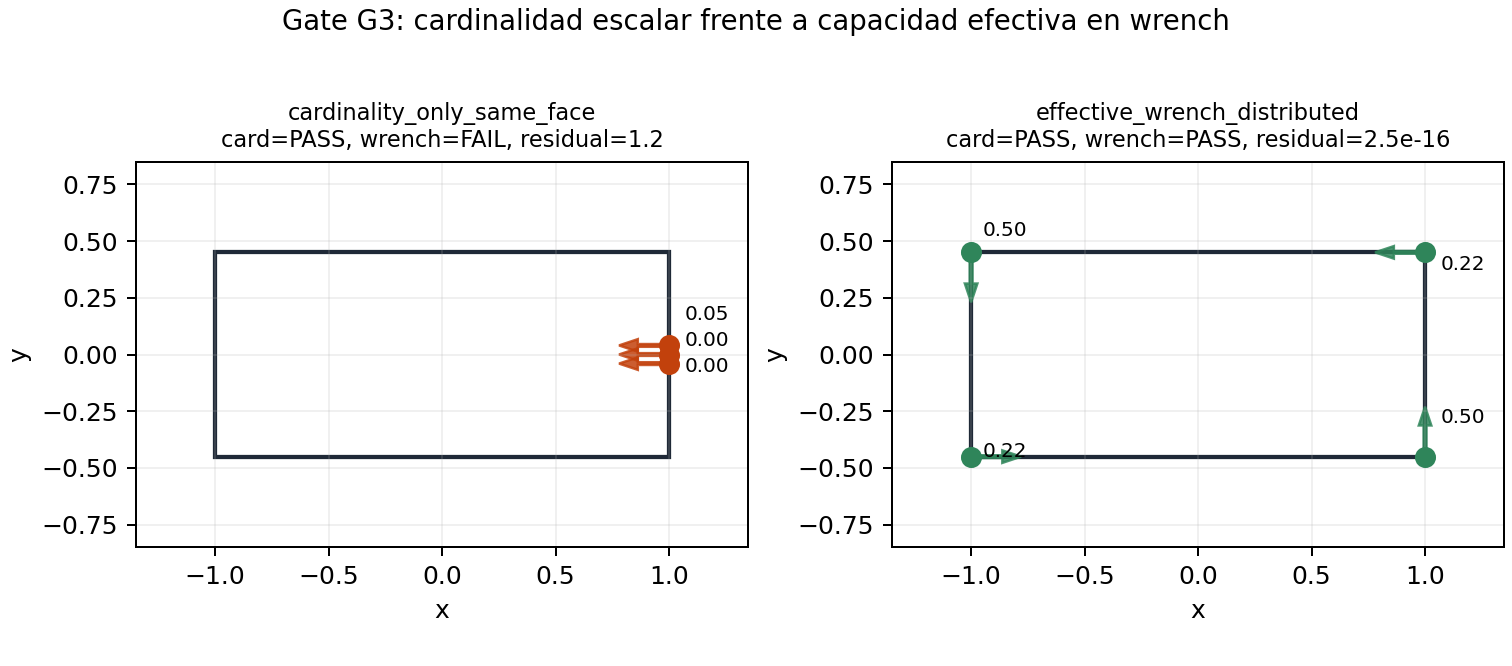
\includegraphics[width=0.92\textwidth]{figures/fig-wrench-capacity-gate.png}
\caption{Gate G3. A la izquierda, el criterio de cardinalidad acepta una coalición
incapaz de producir el par demandado; a la derecha, la distribución de contactos restaura
el rango planar y hace factible el wrench.}
\label{fig:wrench-capacity-gate}
\end{figure}

La conclusión no depende de una escena compleja. Incluso con el mismo objeto y la misma
demanda, $|\mathcal C_k|\geq n_k$ puede declarar una tarea cerrada mientras
\eqref{eq:ctrl_deficit_wrench_socp} devuelve un residual físico positivo. Esta es la
razón matemática para sustituir capacidad escalar por capacidad efectiva en espacio
wrench cuando el transporte exige torque, giro alrededor de obstáculos o contacto
anisotrópico.

El gate G4 añade una auditoría de coherencia del motor matemático completo. No simula una misión industrial
completa; comprueba que las conexiones algebraicas mínimas del framework no son
decorativas. El test evalúa nueve invariantes: firma de torque de círculo, cuadrado y
rectángulo; separación entre fase útil para fuerza y fase útil para torque; desplazamiento
de fase por peaje de congestión; penalización de batería en el mercado; balance de
potencia port-Hamiltoniano; y decaimiento pasivo con entrada nula.

\begin{table}[H]
\centering
\caption{Gate G4: consistencia del motor matemático integrado.}
\label{tab:gate-integrated-math-engine}
\small
\begin{tabularx}{\textwidth}{@{}>{\raggedright\arraybackslash}Xrrc@{}}
\toprule
Chequeo & Observado & Umbral & Estado \\
\midrule
Torque radial nulo en círculo & $0.0000$ & $\le 10^{-8}$ & Pasa \\
Torque no nulo en cuadrado superelíptico & $0.5240$ & $\ge 0.25$ & Pasa \\
Torque no nulo en rectángulo superelíptico & $1.0856$ & $\ge 0.65$ & Pasa \\
Separación fase fuerza--fase torque & $1.0167$ rad & $\ge 0.35$ rad & Pasa \\
Peaje desplaza fase en rectángulo & $3.1416$ rad & $\ge 0.20$ rad & Pasa \\
Peaje desplaza fase en cuadrado & $1.5708$ rad & $\ge 0.20$ rad & Pasa \\
Penalización de batería ordena payoffs & $0.7500$ & $\ge 0.50$ & Pasa \\
Error de balance port-Hamiltoniano & $2.22\cdot10^{-16}$ & $\le 10^{-9}$ & Pasa \\
Derivada pasiva con entrada nula & $0.0000$ & $\le 10^{-9}$ & Pasa \\
\bottomrule
\end{tabularx}
\end{table}

\begin{figure}[H]
\centering
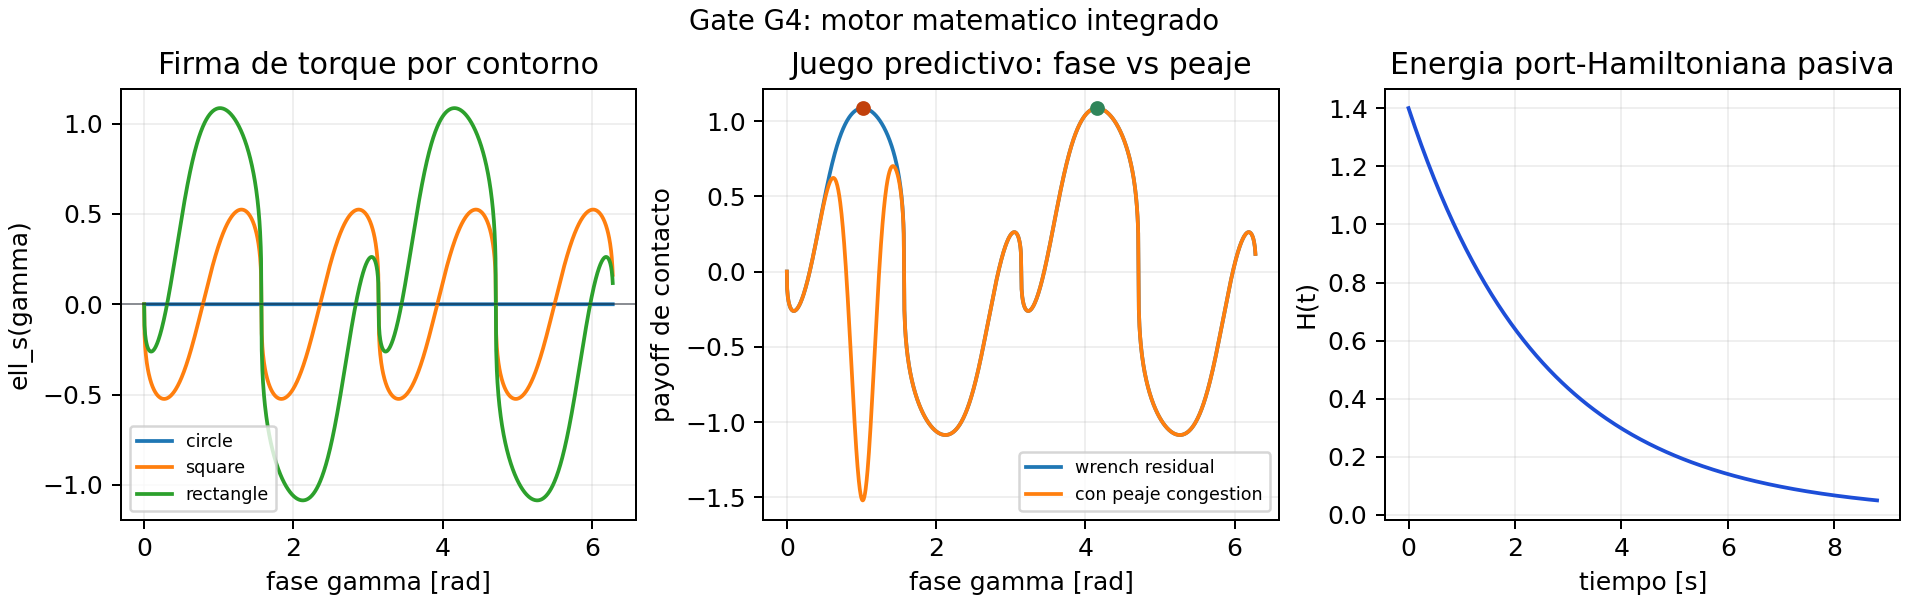
\includegraphics[width=\textwidth]{figures/fig-integrated-math-engine-gate.png}
\caption{Gate G4. Izquierda: la firma de torque distingue círculo, cuadrado y
rectángulo. Centro: el peaje predictivo mueve la fase de contacto hacia otra región útil
antes de que la congestión se materialice. Derecha: la energía port-Hamiltoniana decae
con entrada nula, como exige la pasividad.}
\label{fig:integrated-math-engine-gate}
\end{figure}

La lectura del G4 es que el motor ya no asigna robots a tareas en abstracto. Asigna
contribuciones vectoriales: fuerza, torque, margen de batería y ocupación futura. Si el
residual dominante es fuerza, el mercado escoge una fase frontal; si el residual dominante
es torque, escoge una fase con brazo de palanca; si esa fase se congestiona, el peaje
predictivo desplaza la decisión a otra fase con utilidad mecánica. Esta evidencia no
reemplaza una campaña física completa, pero sí cierra el punto lógico que faltaba:
geometría, mercado, campo y Hamiltoniano consumen la misma señal de déficit.

\subsection{Campañas aplicadas de densidad predictiva, motor integrado y CoppeliaSim}
\label{subsec:campanas-cumlaude}

La suite extendida añade tres campañas reproducibles que convierten parte del marco
avanzado en evidencia experimental. H10 evalúa densidad predictiva en un cuello de
botella de almacén; H11 ejecuta un tramo dinámico con carga rectangular, wrench,
energía, CBF y batería; H12 exporta escenarios CoppeliaSim con cámaras de auditoría y
render sintético de respaldo cuando no se ejecuta el simulador en modo headless.

En H10, Smith-QR con densidad predictiva reduce los pasos congestionados frente a
Smith-QR base con delta medio $-161.7$ pasos e IC95 $[-165.0,-158.4]$. También reduce la
densidad futura máxima en el cuello de botella con delta medio $-17.36$ e IC95
$[-17.52,-17.21]$. La captura de recompensa se mantiene no inferior: la captura media
del tratamiento predictivo es $1.000$ bajo el margen de no inferioridad del $3\%$. La
lectura experimental es que el peaje no sólo existe algebraicamente: bifurca el flujo
hacia la ruta alternativa antes del atasco.

\begin{figure}[H]
\centering
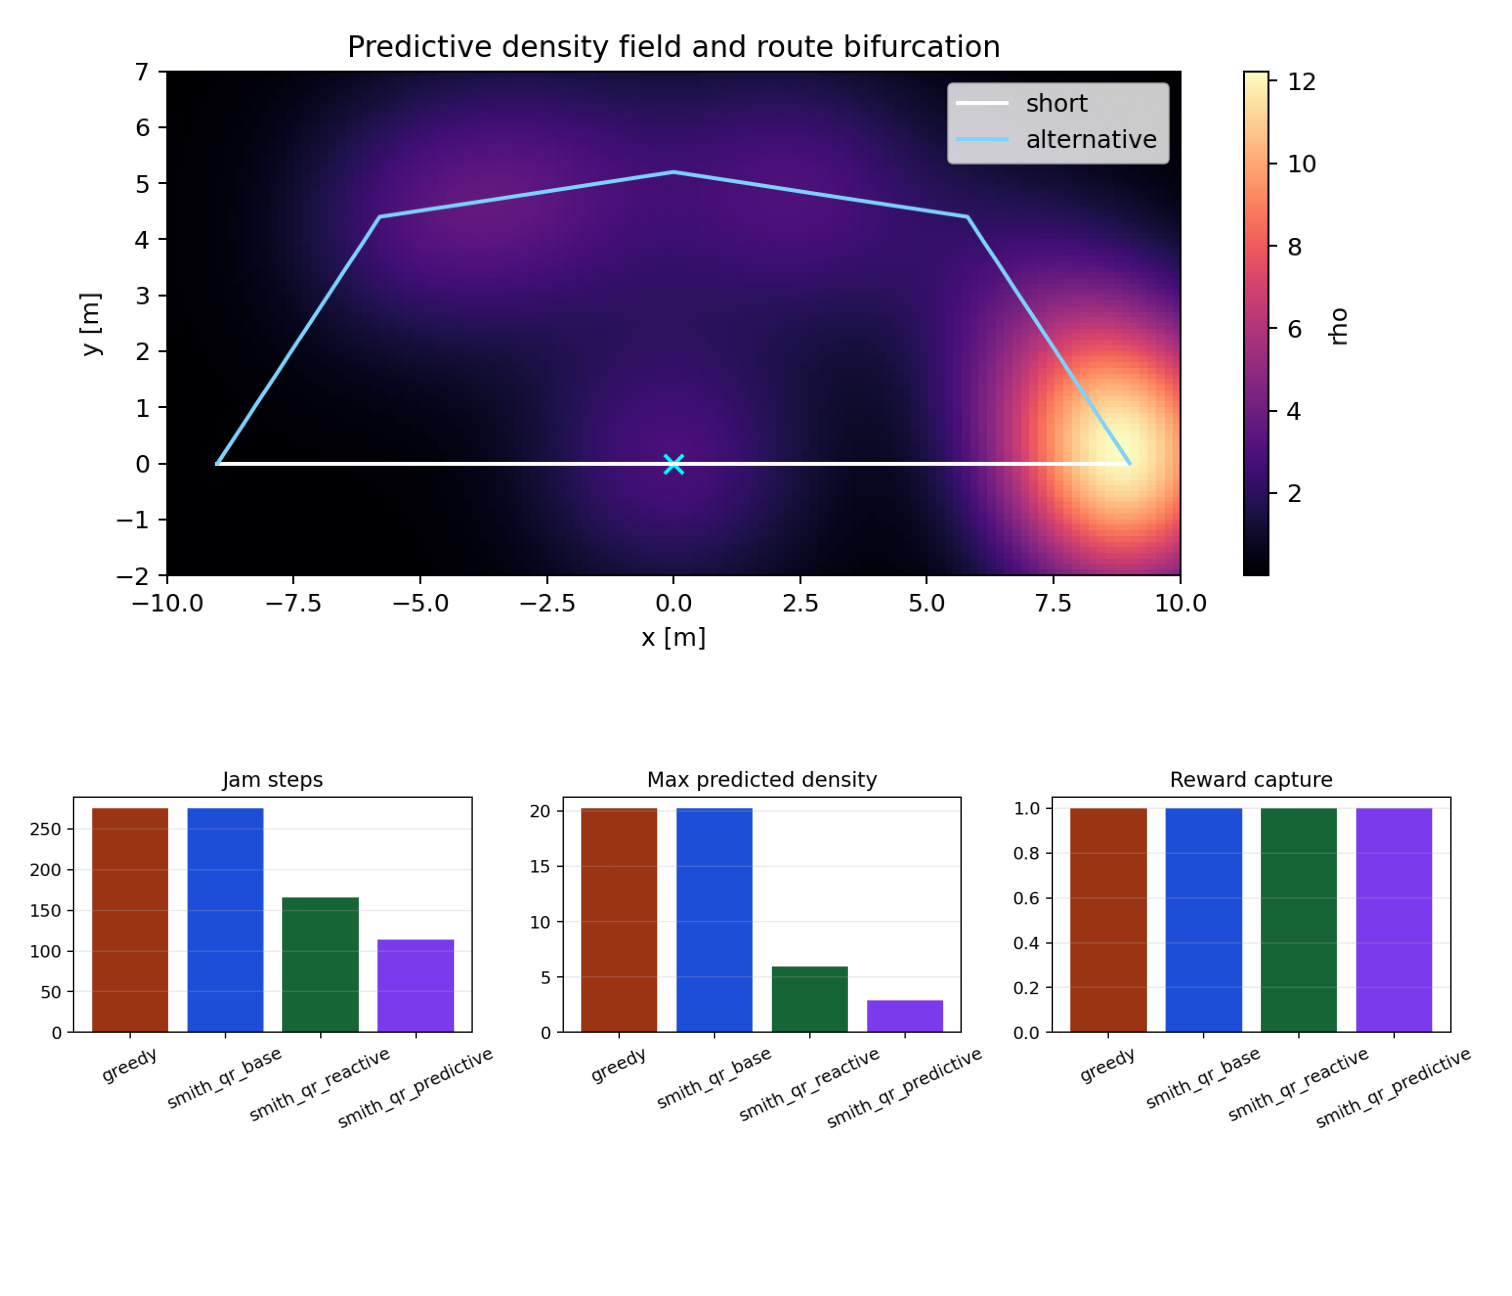
\includegraphics[width=\textwidth]{figures/fig-h10-predictive-density.png}
\caption{Campaña H10. Arriba: mapa de densidad suavizada y bifurcación de rutas.
Abajo: comparación de pasos congestionados, densidad futura máxima y captura de
recompensa.}
\label{fig:h10-predictive-density}
\end{figure}

En H11, la política con capacidad wrench reduce el residual medio frente a cardinalidad
simple con delta $-0.6351$ e IC95 negativo. Además mantiene cotas operativas: la cota
superior IC95 de saturación de torque es $0.4055$ frente al límite $0.85$, la cota
superior IC95 del salto Hamiltoniano es $0.2141$ frente al límite $0.35$, y la cota
inferior IC95 de batería mínima queda por encima de $0.75$. El resultado separa dos
cosas que el conteo escalar confunde: tener suficientes robots y tener robots en fases
de contacto físicamente útiles.

\begin{figure}[H]
\centering
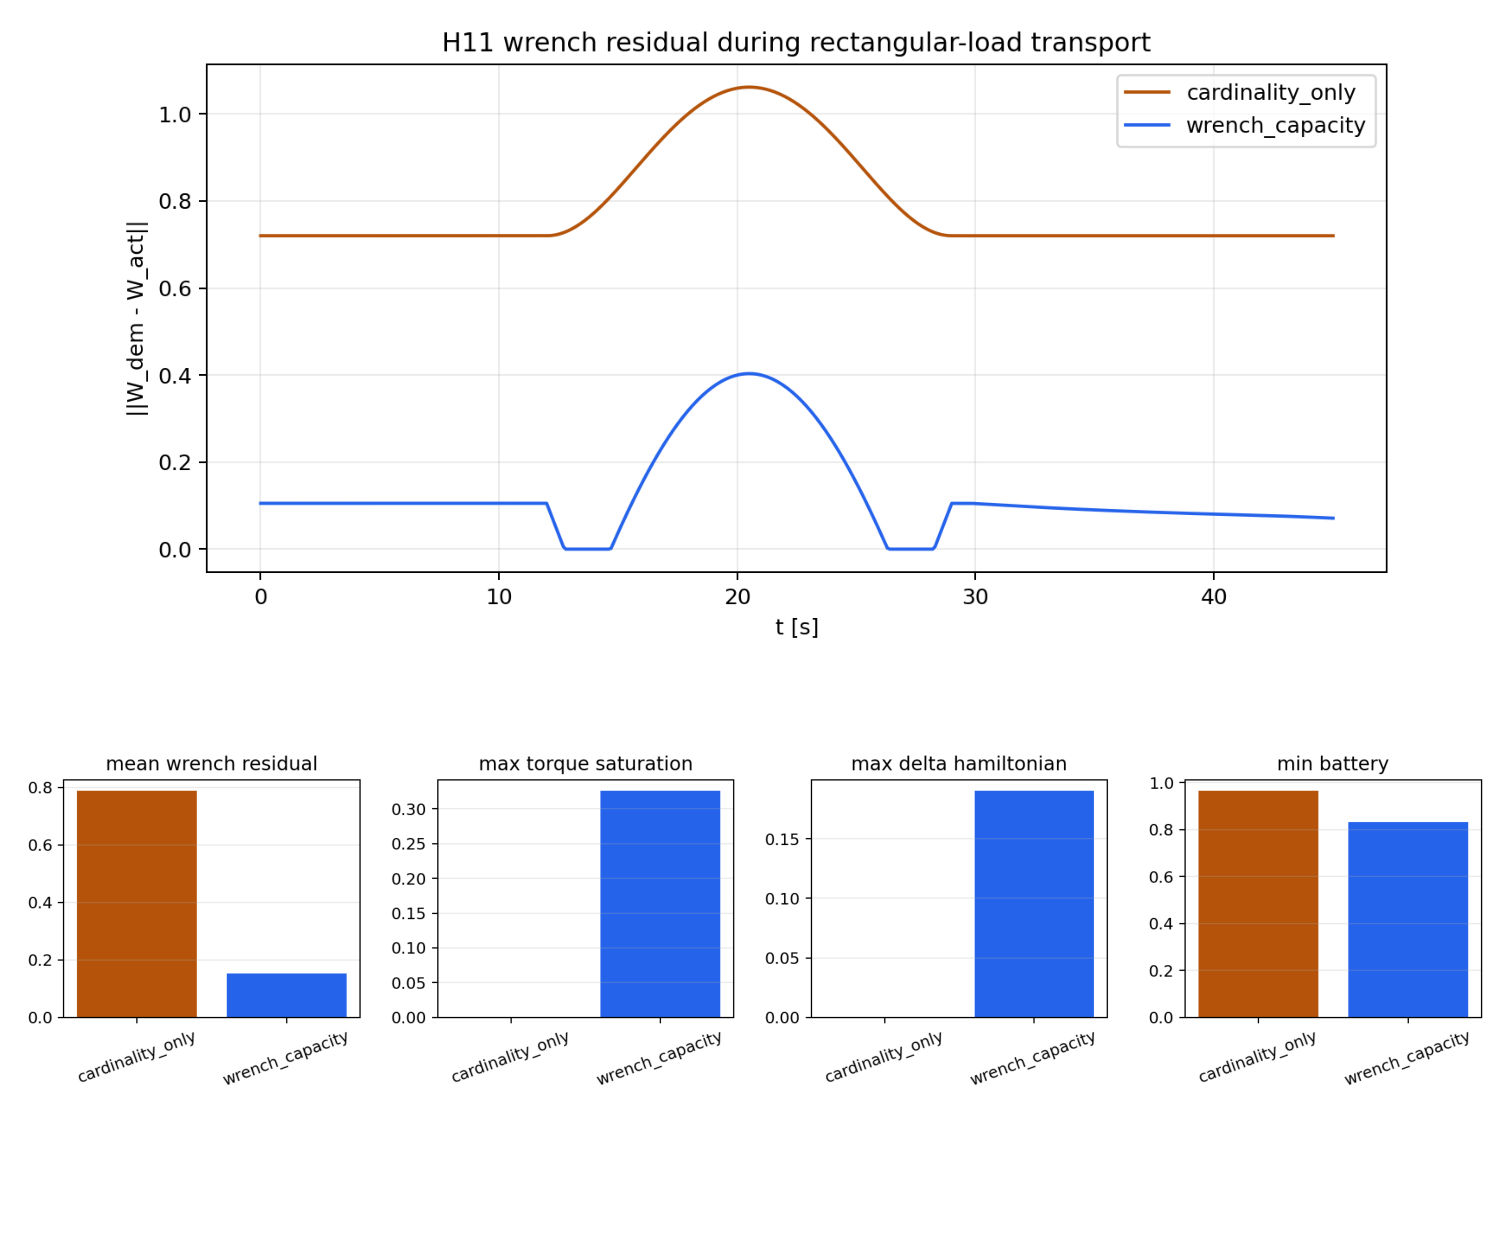
\includegraphics[width=\textwidth]{figures/fig-h11-integrated-engine.png}
\caption{Campaña H11. La capacidad wrench reduce el residual físico durante el tramo
crítico y mantiene torque, energía y batería dentro de cotas operativas.}
\label{fig:h11-integrated-engine}
\end{figure}

En H12 se generan diez escenarios CoppeliaSim: nominal, R3 con Smith, R3 con Smith-QR,
fallo de robot, cruce humano, sensor degradado, cuello de botella con densidad
predictiva, carga rectangular con wrench, batería baja con retorno y escenario integrado.
Cada escena exporta Lua/JSON, playback CSV, cámara superior, cámara oblicua, PNG y MP4
de respaldo. El estado se declara como \emph{fallback synthetic render}: hay cobertura
visual trazable y escenas listas para abrir, pero no se afirma ejecución headless real de
CoppeliaSim.

\begin{figure}[H]
\centering
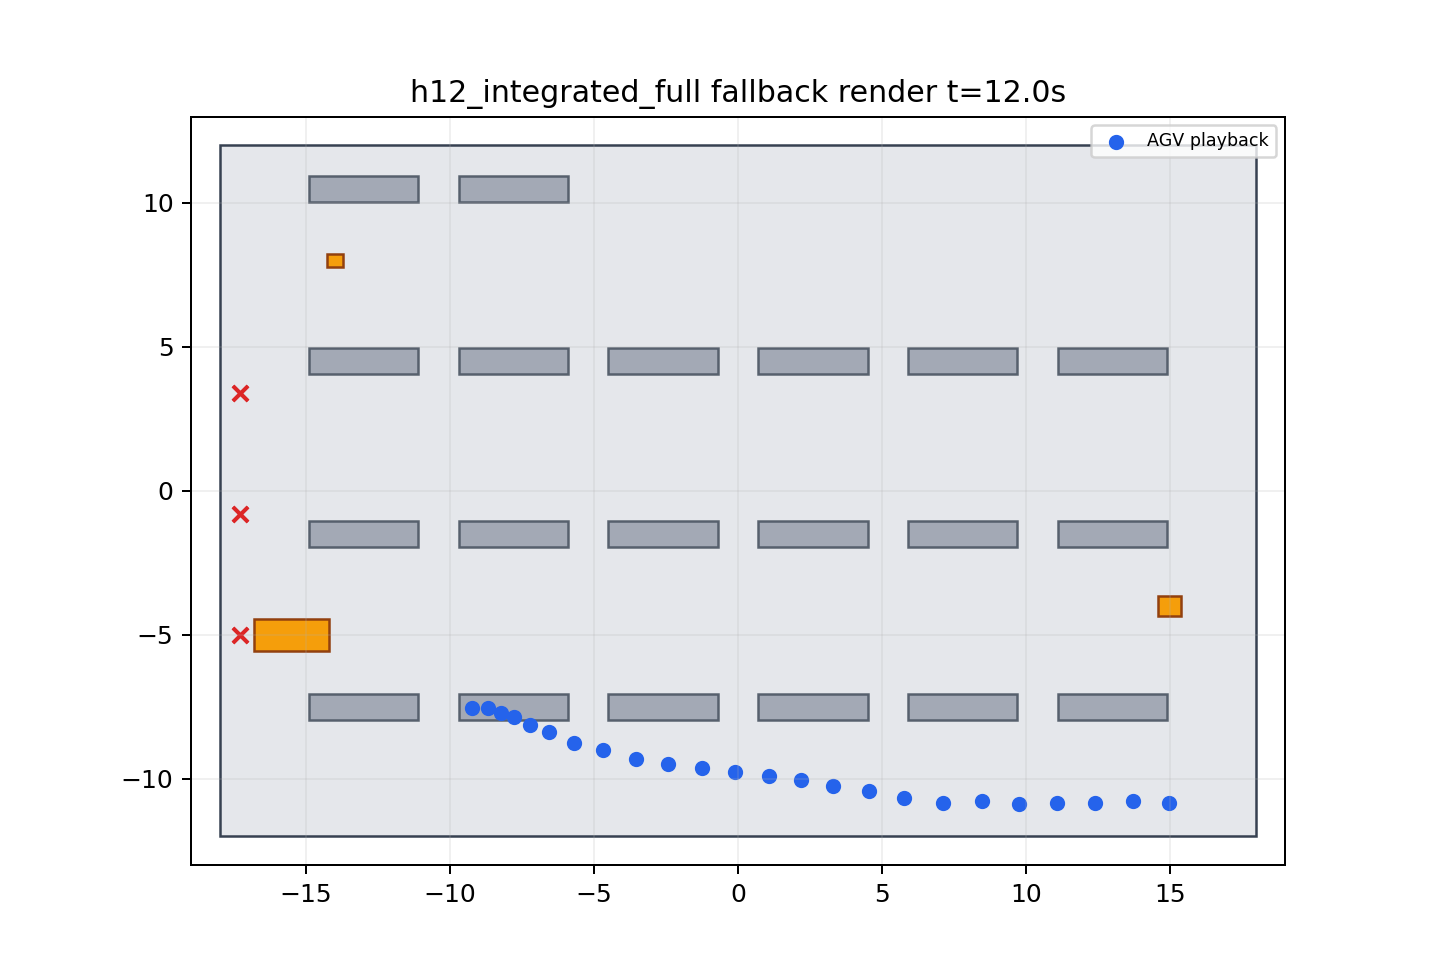
\includegraphics[width=0.92\textwidth]{figures/fig-h12-coppelia-fallback.png}
\caption{Campaña H12. Vista superior de respaldo del escenario integrado, con racks,
robots, cargas y trayectorias de playback.}
\label{fig:h12-coppelia-fallback}
\end{figure}

La validación de escalabilidad se divide en dos niveles. El nivel que sí cierra el
puente teórico es el barrido de aproximación determinista del
Teorema~\ref{teo:aproximacion_determinista_smith}: para
$N\in\{6,12,24,48,96\}$ se compara la ocupación empírica $X^N(t)$ con la ODE
\eqref{eq:ode_smith_fluida}. La Figura~\ref{fig:smith-deterministic-sweep} usa
$N^{-1/2}$ como referencia conservadora; pendientes más negativas indican concentración
más rápida en ese caso homogéneo. El nivel MFG aplicado se abre con H10: el mapa de
densidad suavizada y su predicción corta $\rho(x,t+\tau)$ se usan como peaje virtual de
congestión. Queda pendiente ampliar esta línea a escalados mayores de $N$ y medir de
forma sistemática el coste local $C_{\mathrm{ctrl}}(N)$, pero la primera campaña ya
comprueba que el peaje reduce deadlocks y densidad futura en un cuello de botella
controlado.

El capítulo de transporte amorfo queda parcialmente cubierto por H11. El primer tramo
dinámico ya mide si el residual wrench baja, si la energía port-Hamiltoniana permanece
acotada y si la batería conserva margen durante una maniobra con carga rectangular. Lo
que todavía queda fuera de esta campaña es resolver una PDE MFG completa con densidad de
contacto $\rho_{\partial L}$ y transporte óptimo sobre el contorno. Esa extensión debe
comparar si el coste $Q_L$ desplaza masa hacia arcos útiles sin imponer manualmente la
formación.

La interpretación prevista es la siguiente. Si Smith-QR reduce el colapso de quorum en
R3, debería observarse una trayectoria con menos reconfiguraciones bruscas y, por tanto,
menores $\Delta H$ acumulados que Smith original bajo el mismo escenario. Si la carga
rectangular se atasca frente a un obstáculo, el fallo debería aparecer como crecimiento
de $\tau_{\max}$, violaciones de $h(q)$ o pérdida de roles antes de reflejarse en
throughput. Esta lectura define las variables que debe registrar la variante dinámica
para distinguir fallo de asignación, fallo mecánico y fallo de seguridad.

El framework integrado exige una comparación multi-métrica, no una tabla ordenada sólo
por entregas. Para cada tratamiento se reportará el vector
\eqref{eq:vector_metricas_integrado}: productividad, tiempo, distancia, energía total,
esfuerzo de torque, saltos de Hamiltoniano, error de formación, violaciones de seguridad,
batería mínima, brecha frente a la referencia y coste de cómputo local. La comparación
principal debe ser de Pareto; la puntuación escalar \eqref{eq:score_metricas_integrado}
se usará sólo como resumen secundario con pesos declarados antes de la campaña. Esta
decisión evita una conclusión frágil: un método puede entregar más tareas y aun así ser
peor si destruye batería, satura ruedas o rompe la formación.

La batería se validará con dos lecturas. La primera es operacional: ningún robot debería
cruzar $h_i^B<0$ sin relevo o retorno planificado. La segunda es económica: ante dos
robots con igual capacidad efectiva, el payoff integrado \eqref{eq:payoff_integrado}
debe preferir el robot con mayor margen de retorno o menor coste energético previsto. La
evidencia esperada no es sólo una curva de estado de carga, sino un cambio observable de
asignación cuando la vida útil entra en conflicto con throughput inmediato.

\subsection{Lectura experimental}

Los resultados actuales soportan siete afirmaciones limitadas. Primero, el motor mínimo
reproduce H1 y H2 y evita formular H3 como mecanismo estático. Segundo, Smith original se
paraliza en R3 porque su equilibrio distribuido necesita conectividad suficiente para
cerrar quorums enteros. Tercero, Smith-QR mejora ese límite operativo al cambiar a cierre local
de quorum bajo comunicación degradada. Cuarto, greedy, el proxy MARL inicial, el
MARL-CTDE lineal y el actor neuronal aprendido siguen siendo referencias fuertes en distintos regímenes; por tanto,
la contribución defendible no es que Smith-QR domine todo, sino que conserva una lectura
teórica Smith y añade una transición robusta cuando se viola el supuesto de red. Quinto,
la densidad predictiva ya se valida en un cuello de botella sintético mediante H10.
Sexto, la capacidad wrench reduce residual físico y mantiene límites dinámicos en H11.
Séptimo, H12 aporta cobertura visual reproducible de escenarios CoppeliaSim con artefactos
PNG, MP4 y playback, aunque su estado se declara como fallback sintético y no como
ejecución headless cerrada.
